\chapter{Оценка параметров модели}\label{ch:ch2}

\section{Оценка пороупругих коэффициентов}\label{sec:ch2/sec01}

Выяснению физического смысла и способам лабораторного определения пороупругих констант для среды с двойной пористостью посвящен ряд работ~\autocite{berryman2002models, bai1995poromechanical}. Существуют также обобщения пороупругой модели на случай мульти-пористости~\autocite{mehrabian2015gassmann}. Приведем здесь простые оценки относительных значений коэффициентов $b_1$ и $b_2$, модулей $N_{\alpha}$ и $N_{12}$, подвергнув среду одноосному сжатию с нулевой поперечной деформацией. Соответствующая приближенная одномерная эквивалентная схема состоит из двух последовательно соединенных герметичных камер (элементов схемы). В ненапряженном состоянии продольные размеры камер равны $l_1^0$ и $l_2^0$, причем $l_2^0 \ll l_1^0$, как показано на рисунке~\ref{fig:coef1-1}. Торцевые стенки камер могут скользить без трения вдоль горизонтальной оси. Первая камера, играющая роль матрицы, заполнена пороупругой средой с пористостью $n_1$, упругим модулем $E_1$, коэффициентом Био $\alpha_1$ и модулем Био $\widetilde{N}$. Внутри второй камеры, соответствующей магистральным трещинам, находится пружина жесткостью $E_2$ (считаем, что трещины не заполнены ничем, кроме жидкости). Обозначим $\xi_{\alpha} = \frac{l_{\alpha}}{l_1^0 + l_2^0}$ объемные доли матрицы и трещин, так что $\xi_1 + \xi_2 = 1$. Объемные доли флюидов (<<пористости>>) будут равны $\phi_1 = n_1 \xi_1, phi_2 = n_2 \xi_2$. В камеры независимо нагнетаются давления $p_1$ и $p_2$.

\begin{figure}[ht]
    \centerfloat{
        \hfill
        \subcaptionbox[List-of-Figures entry]{\label{fig:coef1-1}}{%
            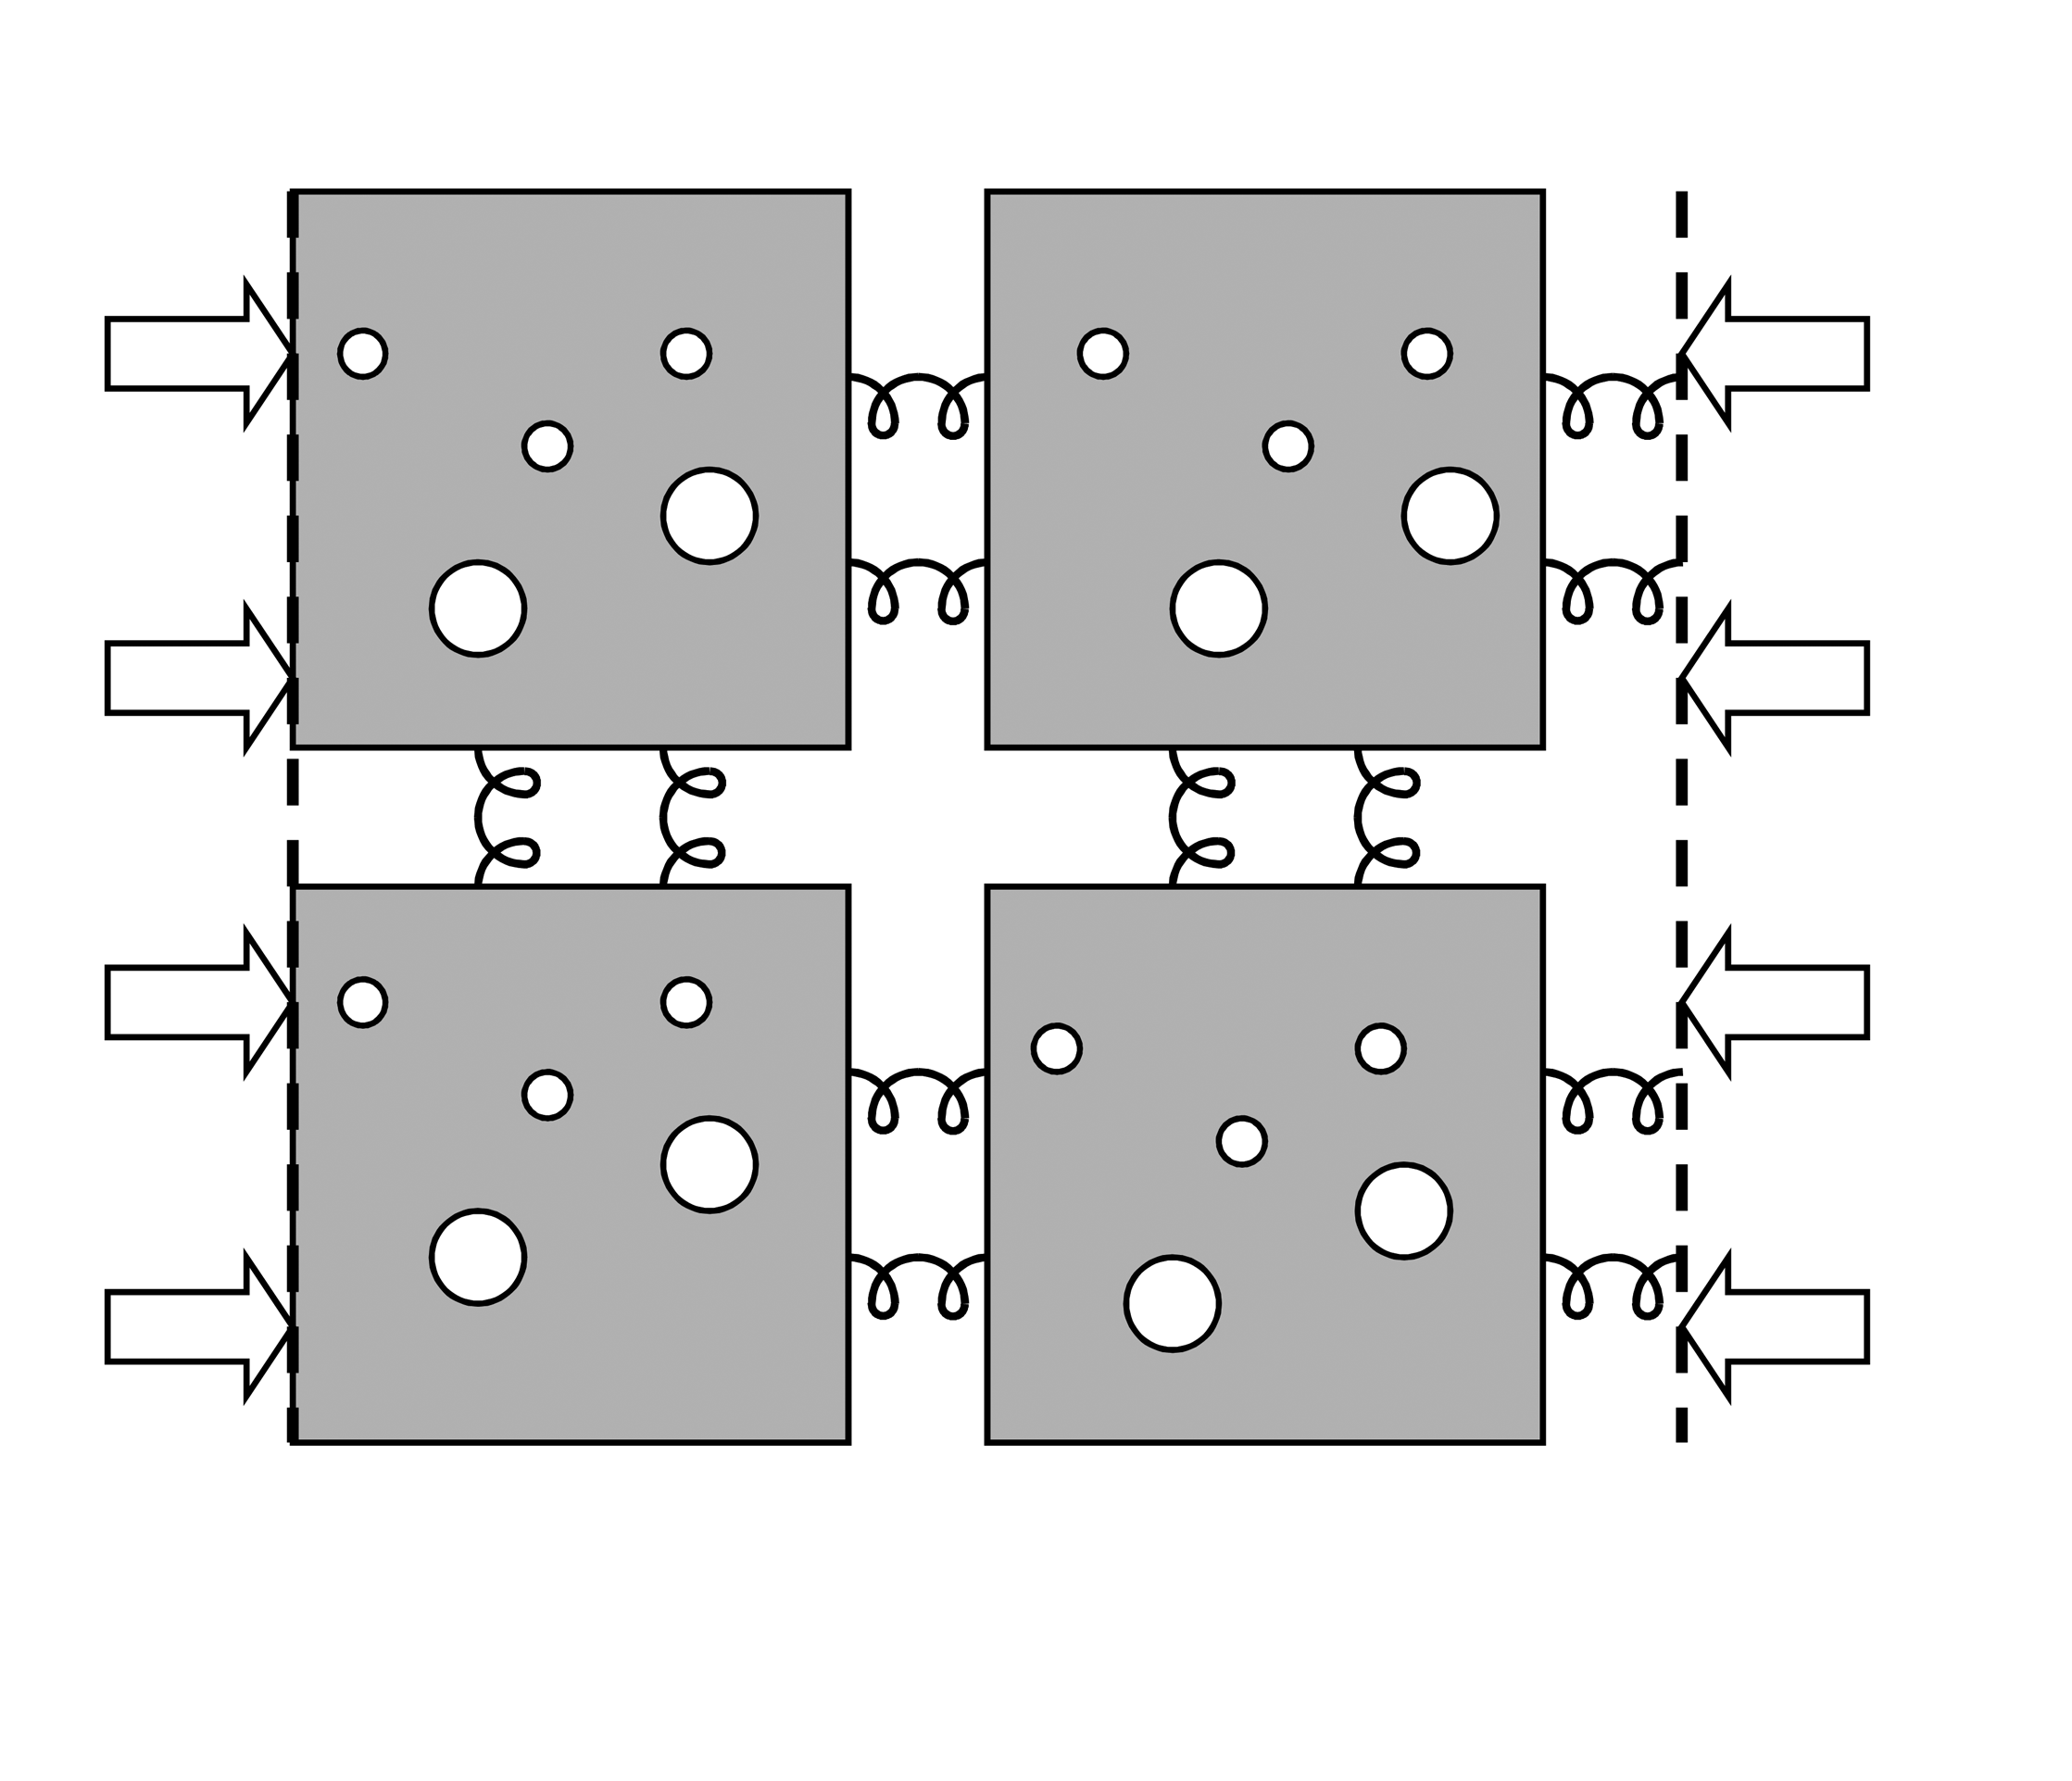
\includegraphics[width=0.4\linewidth]{coef1}}
        \hfill
        \subcaptionbox{\label{fig:coef1-2}}{%
            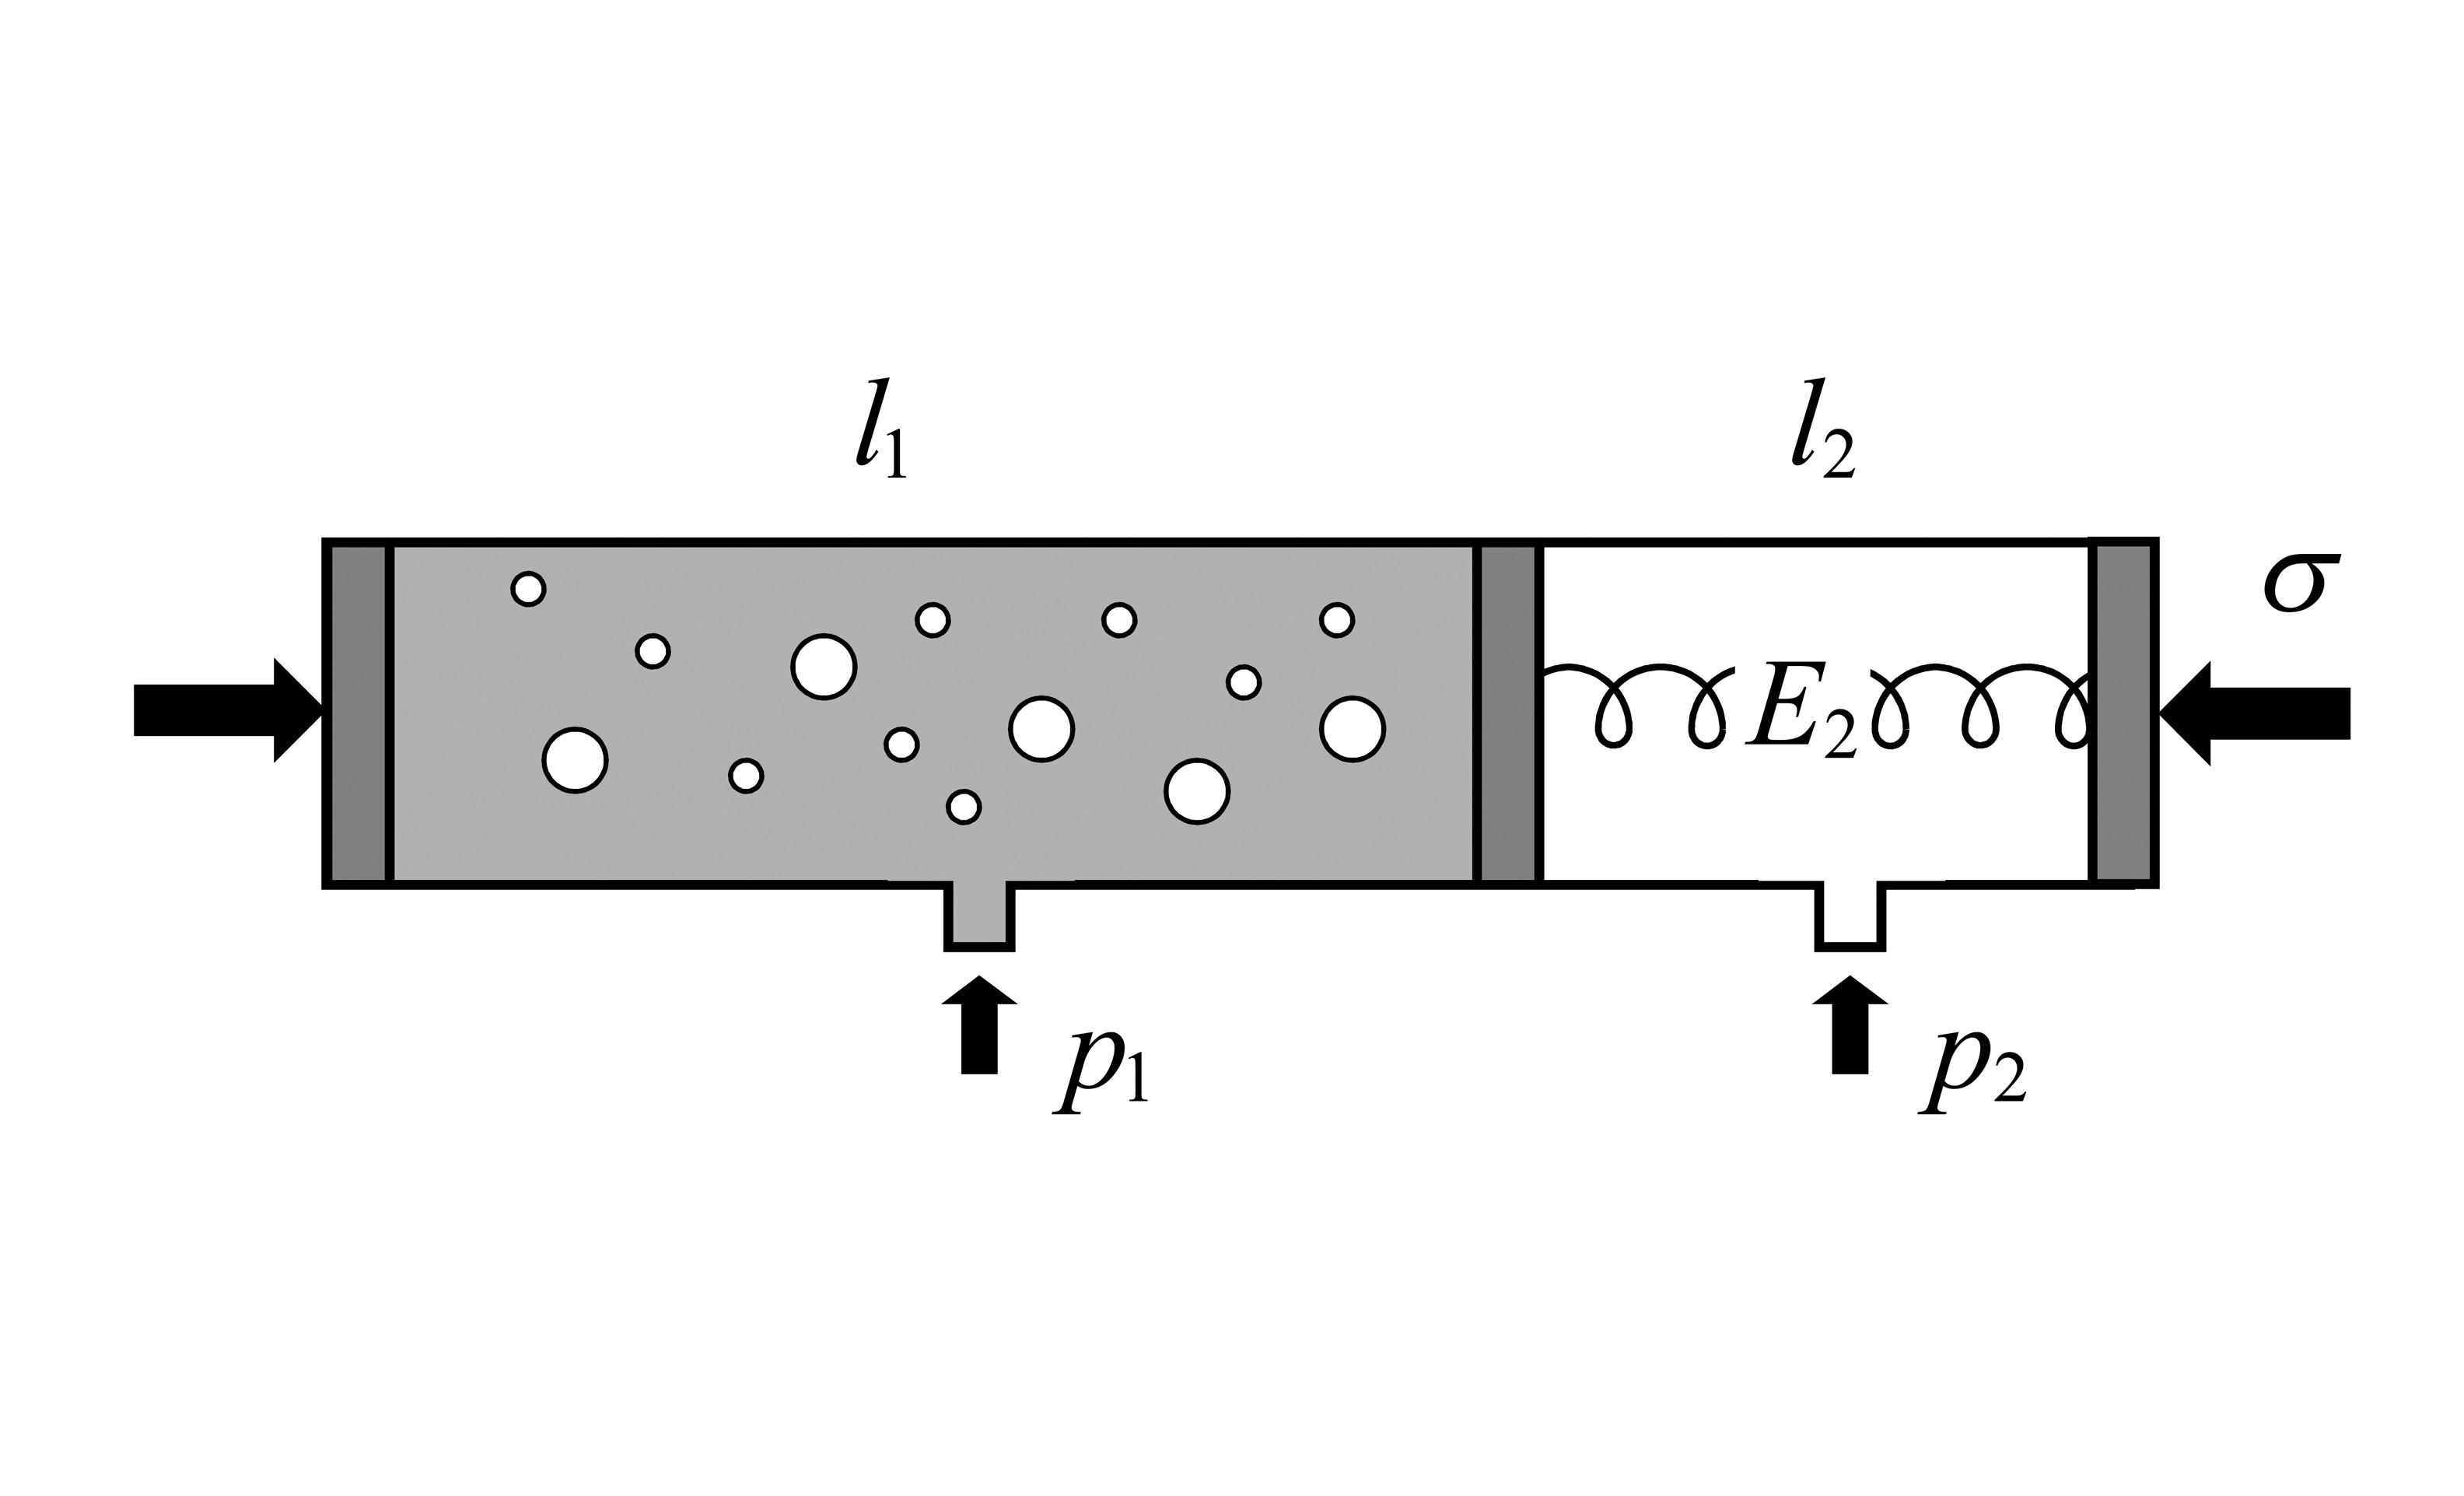
\includegraphics[width=0.6\linewidth]{coef2}}
        \hfill
    }
    % \legend{Упрощенная схема рассматриваемой среды (слева), упрощенная эквивалентная схема (справа).}
    \caption[Упрощенная схема рассматриваемой среды (слева), упрощенная эквивалентная схема (справа).]{Упрощенная схема рассматриваемой среды (слева), упрощенная эквивалентная схема (справа).}\label{fig:coef1}
\end{figure}

Запишем условия равновесия

\begin{equation}
  \label{eq:sigmaeq}
  \sigma = - \alpha_1 p_1 + E_1 \varepsilon_1 = - p_2 + E_2 \varepsilon_2,
\end{equation}
где $\sigma$~--- внешнее сжимающее напряжение, $\varepsilon_{\alpha} = \Delta l_{\alpha} / l_{\alpha}^0$~--- относительные удлинения элементов схемы.

Запишем общую деформацию системы $\varepsilon =  (\Delta l_1 + \Delta l_2) / (l_1^0 + l_2^0)$, как комбинацию относительных удлинений камер

\begin{equation}
  \label{eq:sigmaeq1}
  \varepsilon_{\Sigma} = \varepsilon_1 \xi_1 + \varepsilon_2 \xi_2.
\end{equation}
Выражая относительные удлинения из~\eqref{eq:sigmaeq}, с помощью~\eqref{eq:sigmaeq1} получим аналог закона Гука

\begin{equation}
  \label{eq:sigmaeq2}
  \sigma = E_{\Sigma} \varepsilon_{\Sigma} - \left( \alpha_1 \frac{E_{\Sigma}}{E_1} \xi_1 \right) p_1 + \left( \frac{E_{\Sigma}}{E_2} \xi_2 \right) p_2,
\end{equation}
где $E_{\Sigma} = (\xi_1 / E_1 + \xi_2 / E_2)^{-1}$~--- суммарный упругий модуль системы.

Сравнивая~\eqref{eq:sigmaeq2} с~\eqref{eq:linequationskelet1} в отсутствие поврежденности, приходим к выводу, что коэффициенты при давлениях $p_1$ и $p_2$ играют роль коэффициентов $b_1$ и $b_2$. Таким образом

\begin{equation}
  \label{eq:sigmaeq3}
  \frac{b_1}{b_2} = \frac{\alpha_1 \xi_1}{\xi_2} \frac{E_2}{E_1}.
\end{equation}
При стремлении объемной доли $\xi_2$ к нулю, суммарный упругий модуль системы $E_{\Sigma}$ стремится к $E_1$, а коэффициент $b_1$ стремится к коэффициенту Био матрицы $\alpha_1$. Пусть $\xi_2 \approx 0.01 \xi_1$, тогда при соотношении модулей $E_2/E_1 \approx 10^{-4} - 1$, отношение $b_1/b_2$ будет лежать в диапазоне $10^{-2} - 10^2$.

Модуль $E_2$ определяется, как $E_2 = S_n \Delta \lambda = S_n \xi_2 L$, где $S_n$~--- нормальная жесткость одиночной трещины, $\Delta \lambda$~--- ширина одиночной трещины, $L$~--- характерный размер блока~\autocite{kocharyan2016}.

Возьмем $S_n \approx 10^2$ ГПа/м, $L \approx 1$ м, $E_1 = 10$ ГПа, согласующиеся с данными из Таблиц~\ref{tab:coef1, tab:coef2}, получим, что отношение упругих модулей будет равно $E_2/E_1 \approx 0.1$, тогда согласно~\eqref{eq:sigmaeq3} отношение $b_1/b_2 \approx 10$, а из~\eqref{eq:sigmaeq2} следует $b_1 = 0.9 \alpha_1$, $b_2 = 0.9 \alpha_1$.
Оценим модули $N_{\alpha}$ и $N_{12}$ с помощью предложенной упрощенной схемы. Учитывая, что деформация трещин $\varepsilon_2 = \Delta \phi_2/\phi_2$, деформация матрицы $\varepsilon_1 = \Delta \xi_1 / \xi_1 = \Delta \phi_1 / \phi_1 - \Delta n_1 / n_1$, при этом $\Delta n_1 = alpha_1 \varepsilon_1 + p_1 / \widetilde{N}$ из уравнений~\eqref{eq:sigmaeq} и~\eqref{eq:sigmaeq1} получим оценку

\begin{table} [htbp]%
    \centering
    \caption{}%
    \label{tab:coef1}% label всегда желательно идти после caption
    \renewcommand{\arraystretch}{1.5}%% Увеличение расстояния между рядами, для улучшения восприятия.
    \begin{SingleSpace}
        \begin{tabular}{@{}@{\extracolsep{20pt}}llll@{}} %Вертикальные полосы не используются принципиально, как и лишние горизонтальные (допускается по ГОСТ 2.105 пункт 4.4.5) % @{} позволяет прижиматься к краям
            \toprule     %%% верхняя линейка
            Величина & Значение & Материал \\
            \midrule %%% тонкий разделитель. Отделяет названия столбцов. Обязателен по ГОСТ 2.105 пункт 4.4.5
            $K_f$, ГПа          & 0.5-5~\autocite{craft1959petroleum}         & Нефть   \\
                                &    1.7~\autocite{abousleiman2005poromechanics}        &   \\
            \midrule
            $K_1$, ГПа          & 1.1~\autocite{abousleiman2005poromechanics}           & Сланцы (Gulf of Mexico)    \\
                                &    9.8~\autocite{abousleiman2007geomechanics}        &  Сланцы (Woodford shale) \\
            \midrule
            $\alpha_1$          & 0.96~\autocite{abousleiman2005poromechanics}          & Сланцы (Gulf of Mexico)   \\
            $\xi_2$             & 0.0001–0.01~\autocite{snow1968rock}  &   \\
            \midrule
            $S_n$, ГПа/м                  &    105–117~\autocite{ye2016fracture}      &  Сланцы (Barnett) \\
                                &    226~\autocite{ye2016fracture}       &  Сланцы (Mancos) \\
                                &    25–40~\autocite{ye2016fracture}        &  Сланцы (Pierre) \\
                                \midrule
            $L$, м                    &    0.2–30~\autocite{snow1968rock}        &   \\
            \midrule
            $E_1 = K_1 + \frac{4}{3}\mu $,                     &    2.1~\autocite{abousleiman2005poromechanics}        &  Сланцы (Gulf of Mexico) \\
            ГПа                    &    10–20         &  Сланцы (Woodford shale) \\
                                &    (анизотропия)~\autocite{abousleiman2007geomechanics}       &  \\
                                &    $5.1  \pm 0.5$~\autocite{eseme2007review}        &  Сланцы с высоким \\
                                &           &  содержанием органики \\
                                &    $16.6 \pm 2$~\autocite{eseme2007review}        &  Сланцы с низким \\
                                &           & содержанием органики  \\
                                \midrule
            $n_1$                  &    3.8\%~\autocite{abousleiman2007geomechanics}        &  Сланцы (Woodford shale) \\
                                &    14\%~\autocite{abousleiman2005poromechanics}       &  Сланцы (Gulf of Mexico) \\
                                \midrule
            $\widetilde{N}$, ГПа                    &    27.57~\autocite{abousleiman2005poromechanics}        & Сланцы (Gulf of Mexico)  \\

            \bottomrule %%% нижняя линейка
        \end{tabular}%
    \end{SingleSpace}
\end{table}

\begin{table} [htbp]%
    \centering
    \caption{}%
    \label{tab:coef2}% label всегда желательно идти после caption
    \renewcommand{\arraystretch}{1.5}%% Увеличение расстояния между рядами, для улучшения восприятия.
    \begin{SingleSpace}
        \begin{tabular}{@{}@{\extracolsep{20pt}}llll@{}} %Вертикальные полосы не используются принципиально, как и лишние горизонтальные (допускается по ГОСТ 2.105 пункт 4.4.5) % @{} позволяет прижиматься к краям
            \toprule     %%% верхняя линейка
            Величина & Значение & Материал \\
            \midrule %%% тонкий разделитель. Отделяет названия столбцов. Обязателен по ГОСТ 2.105 пункт 4.4.5
            $\nu$                    &    0.11–0.29       &  Сланцы (Woodford shale) \\
                                &    (анизотропия)~\autocite{abousleiman2007geomechanics}        &  \\
                                &    0.35~\autocite{eseme2007review}        & Сланцы с высоким  \\
                                &           &  содержанием органики \\
                                &    0.2~\autocite{eseme2007review}       &   Сланцы с низким \\
                                &           &  содержанием органики \\

            \bottomrule %%% нижняя линейка
        \end{tabular}%
    \end{SingleSpace}
\end{table}

\begin{table} [htbp]
  \centering
  \begin{threeparttable}% выравнивание подписи по границам таблицы
    \caption{Название таблицы}\label{tab:Ts0Sib}%
    \begin{tabular}{| p{3cm} || p{3cm} | p{7cm} |}
    \hline
    \hline
    Величина & \centering Значение & \centering Материал \\
    \hline
    $K_f$, ГПа      &\centering 0.5-5~\autocite{craft1959petroleum}         &\centering Нефть   \\
                    &\centering    1.7~\autocite{abousleiman2005poromechanics}        &   \\
\hline
    $K_1$, ГПа          &\centering 1.1~\autocite{abousleiman2005poromechanics}           &\centering Сланцы (Gulf of Mexico)    \\
                        &\centering    9.8~\autocite{abousleiman2007geomechanics}        &\centering  Сланцы (Woodford shale) \\
\hline
    $\alpha_1$          &\centering 0.96~\autocite{abousleiman2005poromechanics}          &\centering Сланцы (Gulf of Mexico)   \\
    $\xi_2$             &\centering 0.0001–0.01~\autocite{snow1968rock}  &   \\
\hline
    $S_n$, ГПа/м                  &\centering    105–117~\autocite{ye2016fracture}      &\centering  Сланцы (Barnett) \\
                        &\centering    226~\autocite{ye2016fracture}       &\centering  Сланцы (Mancos) \\
                        &\centering    25–40~\autocite{ye2016fracture}        &\centering  Сланцы (Pierre) \\
\hline
    $L$, м                    &\centering    0.2–30~\autocite{snow1968rock}        &   \\
\hline
    $E_1 = K_1 + \frac{4}{3}\mu $,                     &\centering    2.1~\autocite{abousleiman2005poromechanics}        &\centering  Сланцы (Gulf of Mexico) \\
    ГПа                    &\centering    10–20         &\centering  Сланцы (Woodford shale) \\
                        &\centering    (анизотропия)~\autocite{abousleiman2007geomechanics}       &  \\
                        &\centering    $5.1  \pm 0.5$~\autocite{eseme2007review}        &\centering  Сланцы с высоким \\
                        &\centering           &\centering  содержанием органики \\
                        &\centering    $16.6 \pm 2$~\autocite{eseme2007review}        &\centering  Сланцы с низким \\
                        &\centering           &\centering содержанием органики  \\
\hline
    $n_1$                  &\centering    3.8\%~\autocite{abousleiman2007geomechanics}        &\centering  Сланцы (Woodford shale) \\
                        &\centering    14\%~\autocite{abousleiman2005poromechanics}       &\centering  Сланцы (Gulf of Mexico) \\
\hline
    $\widetilde{N}$, ГПа                    &\centering    27.57~\autocite{abousleiman2005poromechanics}        &\centering Сланцы (Gulf of Mexico)  \\


    \hline
    \hline
    \end{tabular}
  \end{threeparttable}
\end{table}

\begin{equation}
  \label{eq:sigmaeq4}
  \frac{1}{N_1} = \frac{(\alpha_1 - b_1) (  + \alpha_1/n_1) \phi_1}{E_1} + \frac{\phi_1}{n_1 \widetilde{N}},
\end{equation}

\begin{equation}
  \label{eq:sigmaeq5}
  \frac{1}{N_2} = \frac{(1 - b_2) \phi_2}{E_2},
\end{equation}

\begin{equation}
  \label{eq:sigmaeq6}
  \frac{1}{N_{12}} = - \frac{b_1 \phi_2}{E_2}.
\end{equation}
Тогда для относительных величин справедливо

\begin{equation}
  \label{eq:sigmaeq7}
  \frac{N_2}{N_1} = \frac{1}{(1-b_2)} \left( (\alpha_1 - b_1) \left( 1 + \frac{\alpha_1}{n_1} \right) + \frac{E_1}{n_1 \widetilde{N}} \right) \frac{b_1}{b_2},
\end{equation}

\begin{equation}
  \label{eq:sigmaeq8}
  \frac{N_2}{N_{12}} = - \frac{b_1}{1 - b_2}.
\end{equation}

При $b_1/b_2 \approx 10$ и $\alpha_1 = 0.7$ из~\eqref{eq:sigmaeq8} получим оценку $N_2/N_{12} \approx 0.68$. Если дополнительно положить $n_1 = 0.1$ и $E_1/(n_1 \widetilde{N}) \approx 1$, тогда согласно соотношению~\eqref{eq:sigmaeq7} отношение $N_2/N_1 \approx 16.6$. Таким образом, абсолютные значения модулей  и  в рамках сделанных предположений имеют один порядок и более чем на порядок превышают модуль $N_1$. В последующих расчетах будем придерживаться полученных соотношений.

\section{Оценка параметров в модели поврежденности для матрицы}\label{sec:ch2/sec02}

В предложенную линейную модель поврежденности входит ряд коэффициентов. Оценим их, задавшись гипотезой о частном механизме разрушения матрицы. Обозначим коэффициенты, отвечающие за уменьшение упругой энергии матрицы $\alpha_M$, $\alpha_{JM}$, $\alpha_{pM}$ . В работах~\autocite{engelder1990natural, luo2002natural} указывается, что трещины автофлюидоразрыва развиваются преимущественно за счет нормального раскрытия. Принимая указанный механизм разрушения, положим, что в матрице содержится некоторое количество плоских круглых трещин (penny shaped) диаметром $l$, ориентация которых имеет изотропное распределение. Пренебрежем взаимодействием этих трещин, таким образом, уравнение~\eqref{eq:eq34} при $p_2 = 0$ соответствует условию начала развития одиночной трещины. В отличие от~\autocite{engelder1990natural} будем полагать, что стенки трещин непроницаемы для флюида, что правомерно в условиях сверхнизкой проницаемости.

В случае одноосного сжатия (рисунок~\ref{fig:coef2-1}) под действием внутреннего давления первой раскроется трещина, ориентированная перпендикулярно максимальному сжимающему напряжению $\sigma_V < 0$. Это произойдет при внутреннем давлении $p_{ini}$, равном~\autocite{engelder1990natural}

\begin{figure}[ht]
    \centerfloat{
        \hfill
        \subcaptionbox[List-of-Figures entry]{\label{fig:coef2-1}}{%
            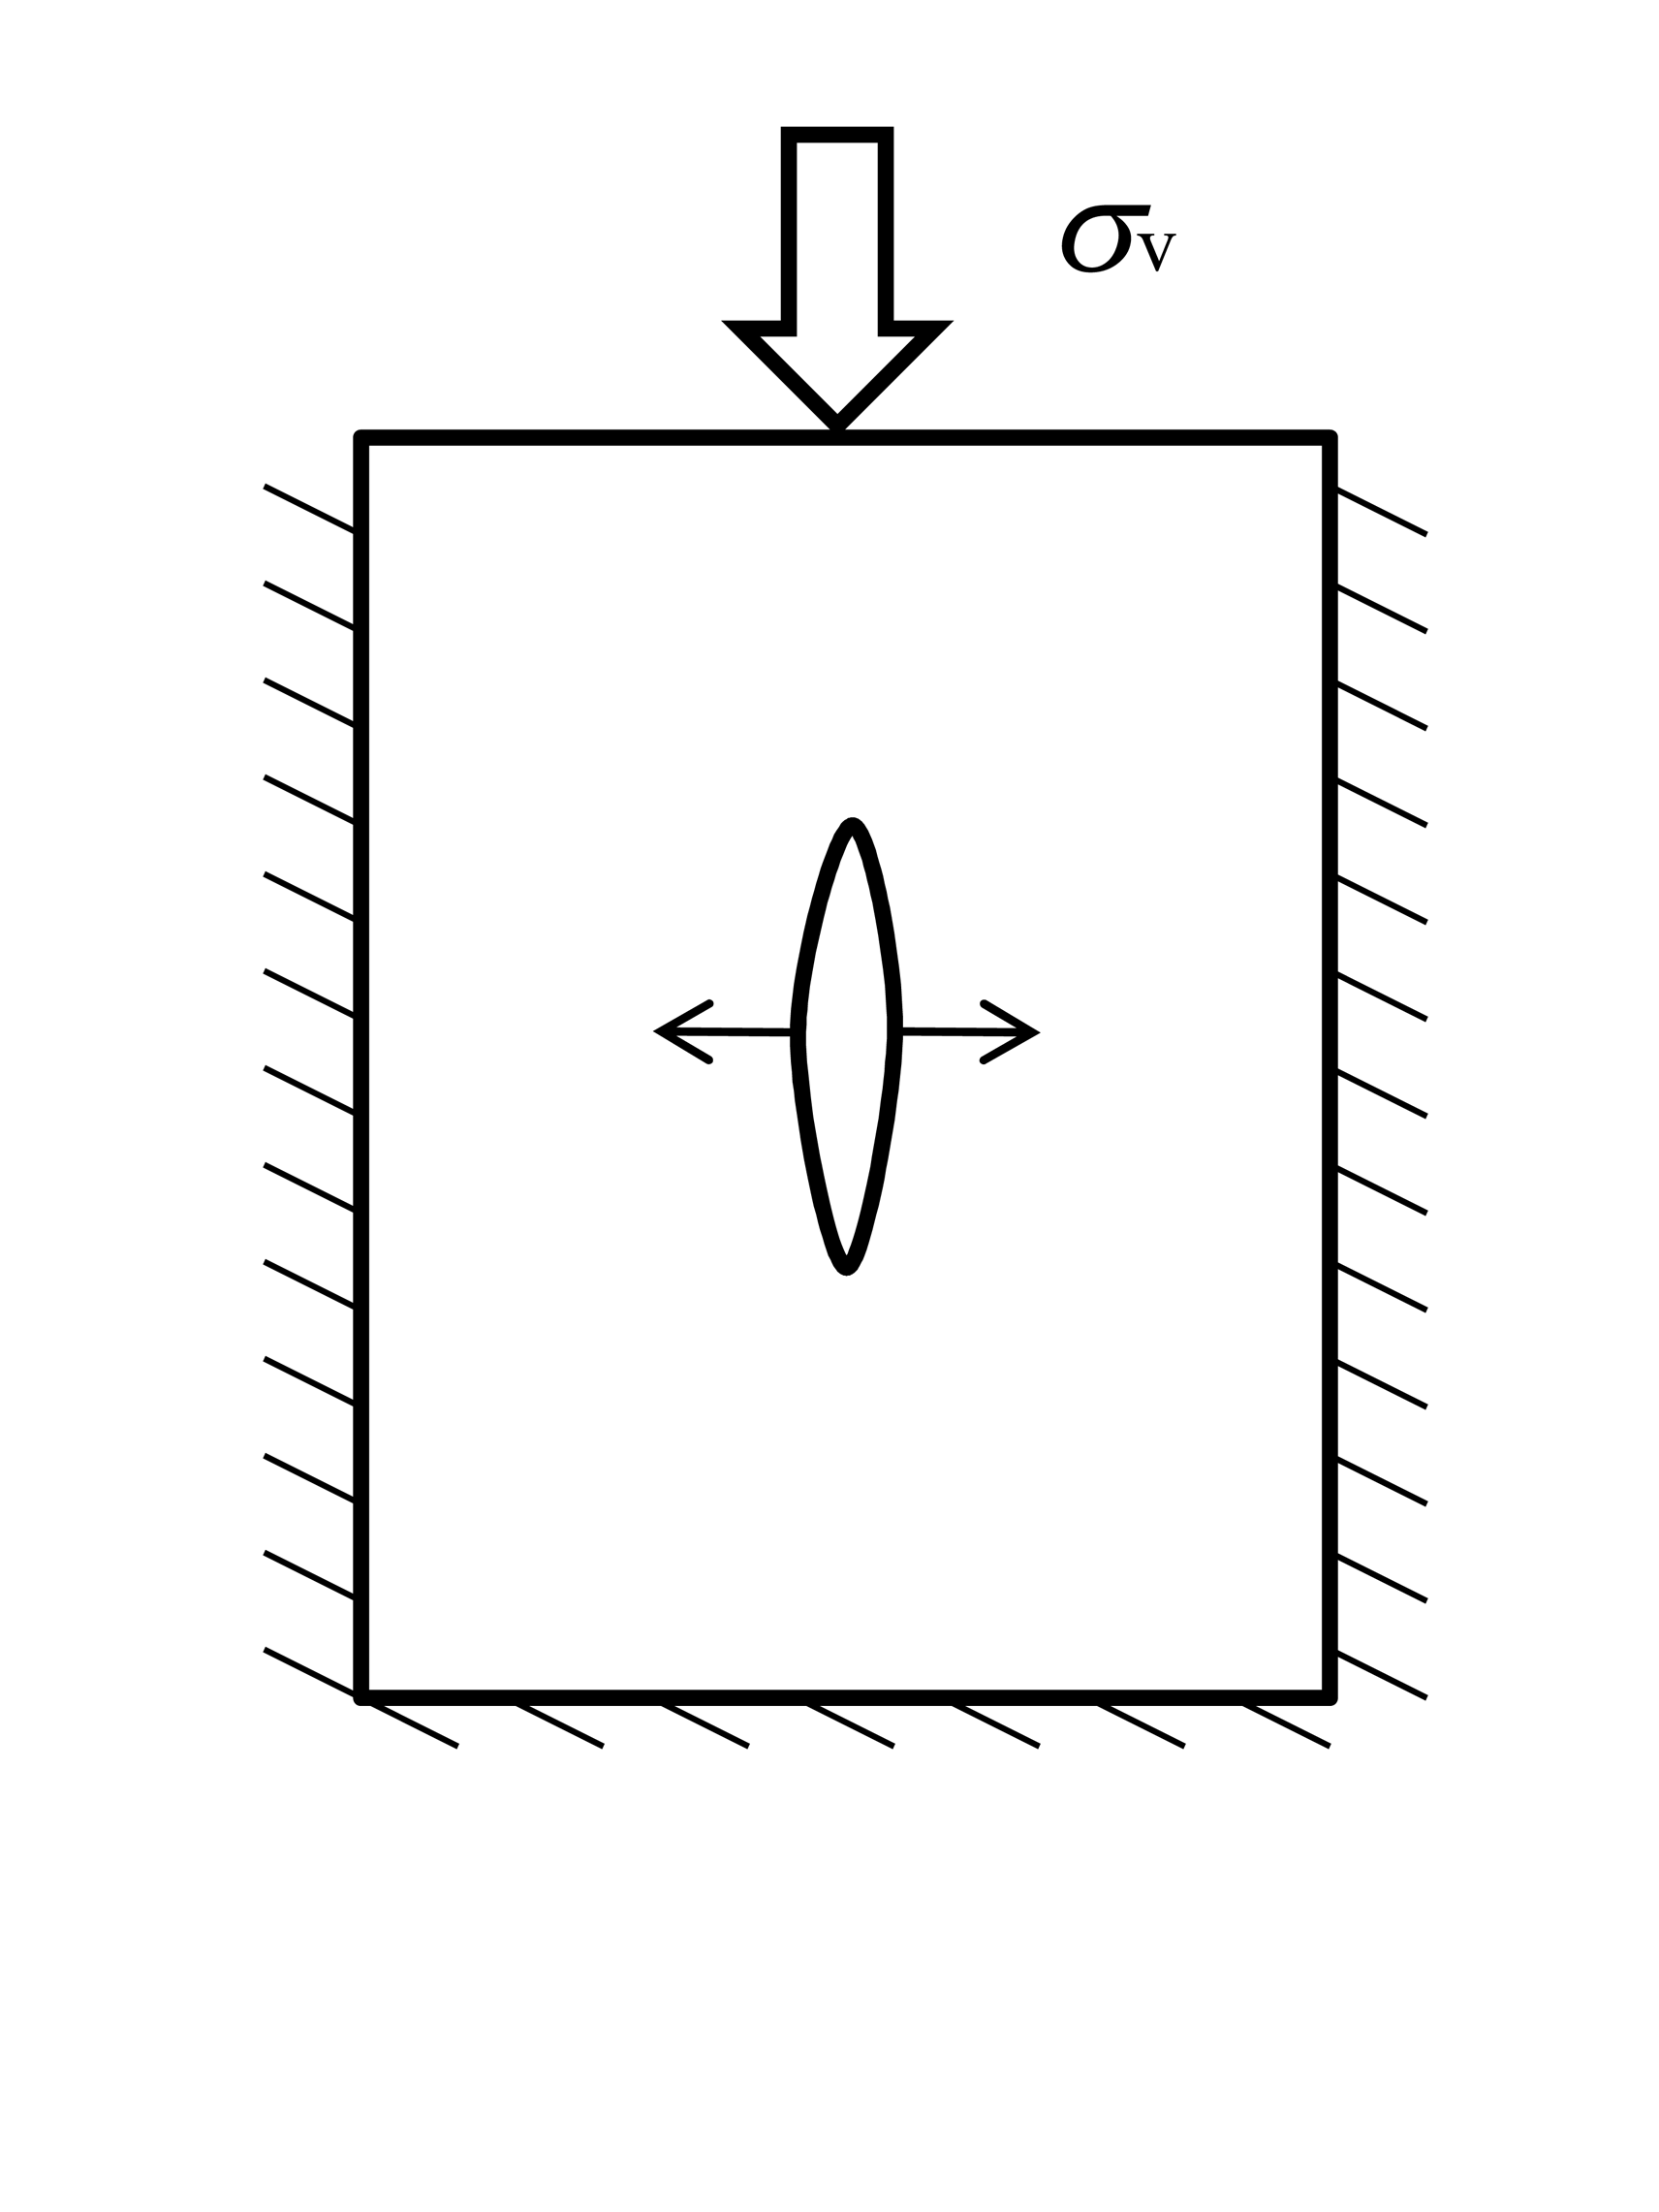
\includegraphics[width=0.4\linewidth]{coef3}}
        \hfill
        \subcaptionbox{\label{fig:coef2-2}}{%
            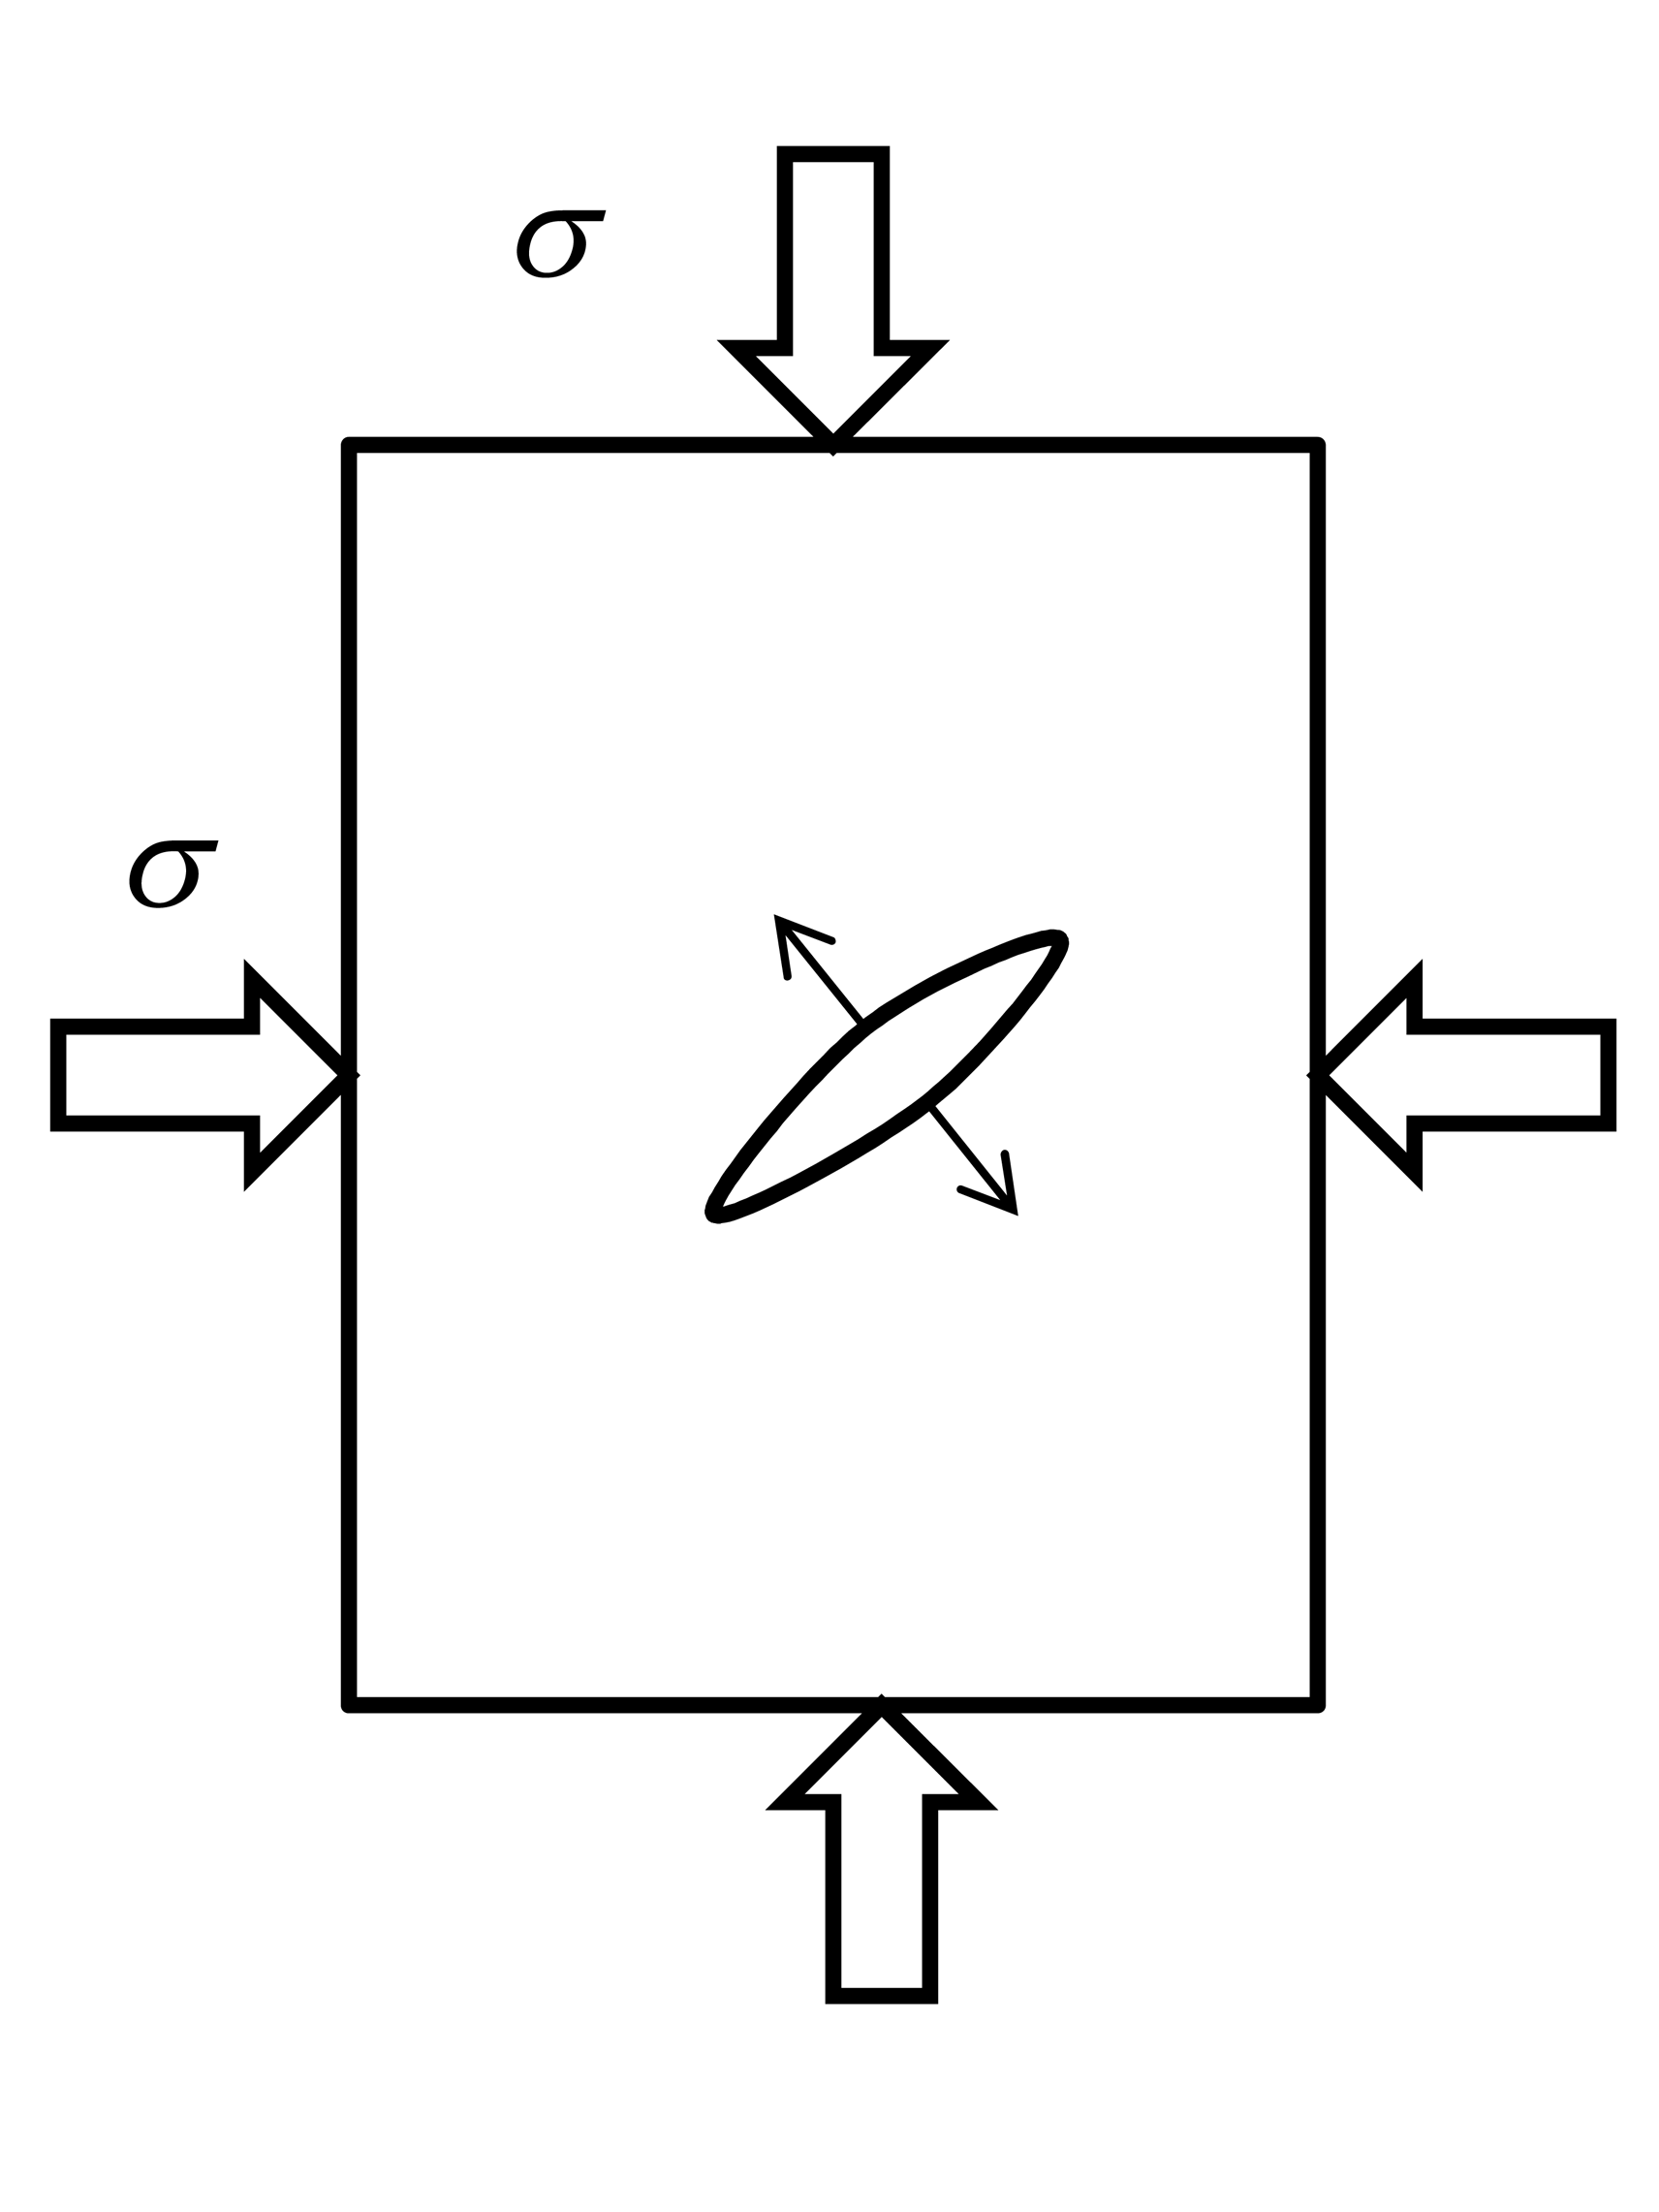
\includegraphics[width=0.4\linewidth]{coef4}}
        \hfill
    }
    % \legend{Одноосное сжатие (слева); гидростатическое сжатие (справа).}
    \caption[Одноосное сжатие (слева); гидростатическое сжатие (справа).]{Одноосное сжатие (слева); гидростатическое сжатие (справа).}\label{fig:coef2}
\end{figure}

\begin{equation}
  \label{eq:omegaeq1}
  p_{ini} = \frac{K_{IC}}{1.13 \sqrt{l}} - \frac{\nu}{1 - \nu }\sigma_V,
\end{equation}
где $\nu$~--- коэффициент Пуассона, $K_{IC}$~--- критический коэффициент интенсивности напряжений при нормальном раскрытии одиночной трещины.

В случае всестороннего сжатия (рисунок~\ref{fig:coef2-2}) уравнение для критического давления будет иметь вид

\begin{equation}
  \label{eq:omegaeq2}
  p_{ini} = \frac{K_{IC}}{1.13 \sqrt{l}} - \sigma.
\end{equation}

Сравнивая~\eqref{eq:linequationskelet5} с~\eqref{eq:linequationskelet2}, получим оценки

\begin{equation}
  \label{eq:omegaeq3}
  \frac{\alpha_{JM}}{\alpha_{PM}} = K,
\end{equation}

\begin{equation}
  \label{eq:omegaeq4}
  \frac{\gamma}{\alpha_{PM}} = \frac{K_{IC}}{1.13 \sqrt{l}}.
\end{equation}

Аналогично рассматривая трещину в условиях одноосного сжатия (в этом случае $J = -\sqrt{2/3}I_1$), получим

\begin{equation}
  \label{eq:omegaeq4}
  \frac{\alpha_{JM}}{\alpha_{M}} = \frac{3 - 7 \nu +2 \nu^2}{\sqrt{6}(1-\nu)^2}.
\end{equation}

В работе~\autocite{grytsenko2010numerical} с помощью численных расчетов методом сингулярных интегральных уравнений было показано, что в случае ансамбля из большого числа одинаковых трещин, находящихся на расстояниях больше либо порядка их длины, критический коэффициент интенсивности напряжений зависит от взаимного расположения трещин, однако отличается от $K_{IC}$ не более чем на $30\%$ (в меньшую сторону).

Параметр $\beta$ в расчетах подбирался таким, чтобы выполнялось неравенство $\alpha_{M}^2 /\beta < K$.

\section{Условие разрушения среды с двойной пористостью}\label{sec:ch2/sec03}

Обратимся теперь к среде с двойной пористостью. Воспользуемся одномерной моделью. Пусть условие начала поврежденности в матрице имеет вид:

\begin{equation}
  \label{eq:destroy1}
  \alpha_M \varepsilon_1 + \alpha_{pM} p_1 - \gamma = 0.
\end{equation}
Требуется переформулировать его в терминах полной деформации $\varepsilon_{\Sigma}$. Исключим  из условия~\eqref{eq:destroy1} с помощью~\eqref{eq:sigmaeq}и~\eqref{eq:sigmaeq1}. В итоге получим

\begin{equation}
  \label{eq:destroy1}
  \frac{\alpha_M }{\xi_1} (1 - b_2) \varepsilon_{\Sigma} + \alpha_M(a_1 p_1 - a_2 p_2) - \alpha_{pM}p_1- \gamma = 0,
\end{equation}
где $a_1=\frac{\xi_2}{\xi_1}\frac{b_1}{E_2}, a_2 = \frac{b_2}{E_1}$.

Сравнивая полученное выражение с~\eqref{eq:eq34}, получим, что

\begin{equation}
  \label{eq:destroy2}
  \alpha = \frac{\alpha_M}{\xi_1} (1 - b_2),
\end{equation}

\begin{equation}
  \label{eq:destroy3}
  \alpha_{p1} = \alpha_{M}a_1+ \alpha_{pM} \geq 0,
\end{equation}

\begin{equation}
  \label{eq:destroy4}
  \alpha_{p2} = - \alpha_{M}a_2 \leq 0.
\end{equation}

Используя ранее сделанные оценки $b_1/b_2 \approx 10$, $E_2/E_1 \approx 0.1$, $\xi_2 \approx 0.01 \xi_1$, получим $a_1 \approx a_2$, $\alpha \approx \alpha_M$. Далее, используя оценку  (одномерный аналог~\eqref{eq:omegaeq3}), получим соотношение между коэффициентами $\alpha_{p_1}$ и $\alpha_{p2}$:

\begin{equation}
  \label{eq:destroy4}
  \alpha_{p2} \approx \alpha_{p_1} b_2 \leq 0.
\end{equation}


% \begin{figure}[ht]
%   \centerfloat{
%     \includegraphics[scale=0.27]{latex}
%   }
%   \caption{TeX.}\label{fig:latex}
% \end{figure}
%
% Для выравнивания изображения по-центру используется команда \verb+\centerfloat+, которая является во
% многом улучшенной версией встроенной команды \verb+\centering+.
%
% \section{Длинное название параграфа, в котором мы узнаём как сделать две картинки с~общим номером и названием}\label{sec:ch2/sect2}
%
% А это две картинки под общим номером и названием:
% \begin{figure}[ht]
%   \begin{minipage}[b][][b]{0.49\linewidth}\centering
%     \includegraphics[width=0.5\linewidth]{knuth1} \\ а)
%   \end{minipage}
%   \hfill
%   \begin{minipage}[b][][b]{0.49\linewidth}\centering
%     \includegraphics[width=0.5\linewidth]{knuth2} \\ б)
%   \end{minipage}
%   \caption{Очень длинная подпись к изображению,
%       на котором представлены две фотографии Дональда Кнута}
%   \label{fig:knuth}
% \end{figure}
%
% Те~же~две картинки под~общим номером и~названием,
% но с автоматизированной нумерацией подрисунков:
% \begin{figure}[ht]
%     \centerfloat{
%         \hfill
%         \subcaptionbox[List-of-Figures entry]{Первый подрисунок\label{fig:knuth_2-1}}{%
%             \includegraphics[width=0.25\linewidth]{knuth1}}
%         \hfill
%         \subcaptionbox{\label{fig:knuth_2-2}}{%
%             \includegraphics[width=0.25\linewidth]{knuth2}}
%         \hfill
%         \subcaptionbox{Третий подрисунок, подпись к которому
%         не~помещается на~одной строке}{%
%             \includegraphics[width=0.3\linewidth]{example-image-c}}
%         \hfill
%     }
%     \legend{Подрисуночный текст, описывающий обозначения, например. Согласно
%     ГОСТ 2.105, пункт 4.3.1, располагается перед наименованием рисунка.}
%     \caption[Этот текст попадает в названия рисунков в списке рисунков]{Очень
%     длинная подпись к второму изображению, на~котором представлены две
%     фотографии Дональда Кнута}\label{fig:knuth_2}
% \end{figure}
%
% На рисунке~\ref{fig:knuth_2-1} показан Дональд Кнут без головного убора.
% На рисунке~\ref{fig:knuth_2}\subcaptionref*{fig:knuth_2-2}
% показан Дональд Кнут в головном уборе.
%
% Возможно вставлять векторные картинки, рассчитываемые \LaTeX\ <<на~лету>>
% с~их~предварительной компиляцией. Надписи в таких рисунках будут выполнены
% тем же~шрифтом, который указан для документа в целом.
% На~рисунке~\ref{fig:tikz_example} на~странице~\pageref{fig:tikz_example}
% представлен пример схемы, рассчитываемой пакетом \verb|tikz| <<на~лету>>.
% Для ускорения компиляции, подобные рисунки могут быть <<кешированы>>, что
% определяется настройками в~\verb|common/setup.tex|.
% Причём имя предкомпилированного
% файла и~папка расположения таких файлов могут быть отдельно заданы,
% что удобно, если не~для подготовки диссертации,
% то~для подготовки научных публикаций.
% \begin{figure}[ht]
%     \centerfloat{
%         \ifdefmacro{\tikzsetnextfilename}{\tikzsetnextfilename{tikz_example_compiled}}{}% присваиваемое предкомпилированному pdf имя файла (не обязательно)
%         \input{Dissertation/images/tikz_scheme.tikz}
%
%     }
%     \legend{}
%     \caption[Пример \texttt{tikz} схемы]{Пример рисунка, рассчитываемого
%         \texttt{tikz}, который может быть предкомпилирован}\label{fig:tikz_example}
% \end{figure}
%
% Множество программ имеют либо встроенную возможность экспортировать векторную
% графику кодом \verb|tikz|, либо соответствующий пакет расширения.
% Например, в GeoGebra есть встроенный экспорт,
% для Inkscape есть пакет svg2tikz,
% для Python есть пакет matplotlib2tikz,
% для R есть пакет tikzdevice.
%
% \section{Пример вёрстки списков}\label{sec:ch2/sec3}
%
% \noindent Нумерованный список:
% \begin{enumerate}
%   \item Первый пункт.
%   \item Второй пункт.
%   \item Третий пункт.
% \end{enumerate}
%
% \noindent Маркированный список:
% \begin{itemize}
%   \item Первый пункт.
%   \item Второй пункт.
%   \item Третий пункт.
% \end{itemize}
%
% \noindent Вложенные списки:
% \begin{itemize}
%   \item Имеется маркированный список.
%   \begin{enumerate}
%     \item В нём лежит нумерованный список,
%     \item в котором
%     \begin{itemize}
%       \item лежит ещё один маркированный список.
%     \end{itemize}
%   \end{enumerate}
% \end{itemize}
%
% \noindent Нумерованные вложенные списки:
% \begin{enumerate}
%   \item Первый пункт.
%   \item Второй пункт.
%   \item Вообще, по ГОСТ 2.105 первый уровень нумерации
%   (при необходимости ссылки в тексте документа на одно из перечислений)
%   идёт буквами русского или латинского алфавитов,
%   а второй "--- цифрами со~скобками.
%   Здесь отходим от ГОСТ.
%     \begin{enumerate}
%       \item в нём лежит нумерованный список,
%       \item в котором
%         \begin{enumerate}
%           \item ещё один нумерованный список,
%           \item третий уровень нумерации не нормирован ГОСТ 2.105;
%           \item обращаем внимание на строчность букв,
%           \item в этом списке
%           \begin{itemize}
%             \item лежит ещё один маркированный список.
%           \end{itemize}
%         \end{enumerate}
%
%     \end{enumerate}
%
%   \item Четвёртый пункт.
% \end{enumerate}
%
% \section{Традиции русского набора}
%
% Много полезных советов приведено в материале
% <<\href{http://www.dropbox.com/s/x4hajy4pkw3wdql/wholesome-typesetting.pdf?dl=1\&pv=1}{Краткий курс благородного набора}>> (автор А.\:В.~Костырка).
% Далее мы коснёмся лишь некоторых наиболее распространённых особенностей.
%
% \subsection{Пробелы}
%
% В~русском наборе принято:
% \begin{itemize}
%     \item единицы измерения, знак процента отделять пробелами от~числа:
%         10~кВт, 15~\% (согласно ГОСТ 8.417, раздел 8);
%     \item \(\tg 20\text{\textdegree}\), но: 20~{\textdegree}C
%         (согласно ГОСТ 8.417, раздел 8);
%     \item знак номера, параграфа отделять от~числа: №~5, \S~8;
%     \item стандартные сокращения: т.\:е., и~т.\:д., и~т.\:п.;
%     \item неразрывные пробелы в~предложениях.
% \end{itemize}
%
% \subsection{Математические знаки и символы}
%
% Русская традиция начертания греческих букв и некоторых математических
% функций отличается от~западной. Это исправляется серией
% \verb|\renewcommand|.
% \begin{itemize}
% %Все \original... команды заранее, ради этого примера, определены в Dissertation\userstyles.tex
%     \item[До:] \( \originalepsilon \originalge \originalphi\),
%     \(\originalphi \originalleq \originalepsilon\),
%     \(\originalkappa \in \originalemptyset\),
%     \(\originaltan\),
%     \(\originalcot\),
%     \(\originalcsc\).
%     \item[После:] \( \epsilon \ge \phi\),
%     \(\phi \leq \epsilon\),
%     \(\kappa \in \emptyset\),
%     \(\tan\),
%     \(\cot\),
%     \(\csc\).
% \end{itemize}
%
% Кроме того, принято набирать греческие буквы вертикальными, что
% решается подключением пакета \verb|upgreek| (см. закомментированный
% блок в~\verb|userpackages.tex|) и~аналогичным переопределением в
% преамбуле (см.~закомментированный блок в~\verb|userstyles.tex|). В
% этом шаблоне такие переопределения уже включены.
%
% Знаки математических операций принято переносить. Пример переноса
% в~формуле~\eqref{eq:equation3}.
%
% \subsection{Кавычки}
% В английском языке приняты одинарные и двойные кавычки в~виде ‘...’ и~“...”.
% В России приняты французские («...») и~немецкие („...“) кавычки (они называются
% «ёлочки» и~«лапки», соответственно). ,,Лапки`` обычно используются внутри
% <<ёлочек>>, например, <<... наш гордый ,,Варяг``...>>.
%
% Французкие левые и правые кавычки набираются
% как лигатуры \verb|<<| и~\verb|>>|, а~немецкие левые
% и правые кавычки набираются как лигатуры \verb|,,| и~\verb|‘‘| (\verb|``|).
%
% Вместо лигатур или команд с~активным символом "\ можно использовать команды
% \verb|\glqq| и \verb|\grqq| для набора немецких кавычек и команды \verb|\flqq|
% и~\verb|\frqq| для набора французских кавычек. Они определены в пакете
% \verb|babel|.
%
% \subsection{Тире}
% %  babel+pdflatex по умолчанию, в polyglossia надо включать опцией (и перекомпилировать с удалением временных файлов)
% Команда \verb|"---| используется для печати тире в тексте. Оно несколько короче
% английского длинного тире. Кроме того, команда задаёт небольшую жёсткую отбивку
% от слова, стоящего перед тире. При этом, само тире не~отрывается от~слова.
% После тире следует такая же отбивка от текста, как и~перед тире. При наборе
% текста между словом и командой, за которым она следует, должен стоять пробел.
%
% В составных словах, таких, как <<Закон Менделеева"--~Клапейрона>>, для печати
% тире надо использовать команду \verb|"--~|. Она ставит более короткое,
% по~сравнению с~английским, тире и позволяет делать переносы во втором слове.
% При~наборе текста команда \verb|"--~| не отделяется пробелом от слова,
% за~которым она следует (\verb|Менделеева"--~|). Следующее за командой слово
% может быть  отделено от~неё пробелом или перенесено на другую строку.
%
% Если прямая речь начинается с~абзаца, то перед началом её печатается тире
% командой \verb|"--*|. Она печатает русское тире и жёсткую отбивку нужной
% величины перед текстом.
%
% \subsection{Дефисы и переносы слов}
% %  babel+pdflatex по умолчанию, в polyglossia надо включать опцией (и перекомпилировать с удалением временных файлов)
% Для печати дефиса в~составных словах введены две команды. Команда~\verb|"~|
% печатает дефис и~запрещает делать переносы в~самих словах, а~команда \verb|"=|
% печатает дефис, оставляя \TeX ’у право делать переносы в~самих словах.
%
% В отличие от команды \verb|\-|, команда \verb|"-| задаёт место в~слове, где
% можно делать перенос, не~запрещая переносы и~в~других местах слова.
%
% Команда \verb|""| задаёт место в~слове, где можно делать перенос, причём дефис
% при~переносе в~этом месте не~ставится.
%
% Команда \verb|",| вставляет небольшой пробел после инициалов с~правом переноса
% в~фамилии.
%
% \section{Текст из панграмм и формул}
%
% Любя, съешь щипцы, "--- вздохнёт мэр, "--- кайф жгуч. Шеф взъярён тчк щипцы
% с~эхом гудбай Жюль. Эй, жлоб! Где туз? Прячь юных съёмщиц в~шкаф. Экс-граф?
% Плюш изъят. Бьём чуждый цен хвощ! Эх, чужак! Общий съём цен шляп (юфть) "---
% вдрызг! Любя, съешь щипцы, "--- вздохнёт мэр, "--- кайф жгуч. Шеф взъярён тчк
% щипцы с~эхом гудбай Жюль. Эй, жлоб! Где туз? Прячь юных съёмщиц в~шкаф.
% Экс-граф? Плюш изъят. Бьём чуждый цен хвощ! Эх, чужак! Общий съём цен шляп
% (юфть) "--- вдрызг! Любя, съешь щипцы, "--- вздохнёт мэр, "--- кайф жгуч. Шеф
% взъярён тчк щипцы с~эхом гудбай Жюль. Эй, жлоб! Где туз? Прячь юных съёмщиц
% в~шкаф. Экс-граф? Плюш изъят. Бьём чуждый цен хвощ! Эх, чужак! Общий съём цен
% шляп (юфть) "--- вдрызг! Любя, съешь щипцы, "--- вздохнёт мэр, "--- кайф жгуч.
% Шеф взъярён тчк щипцы с~эхом гудбай Жюль. Эй, жлоб! Где туз? Прячь юных съёмщиц
% в~шкаф. Экс-граф? Плюш изъят. Бьём чуждый цен хвощ! Эх, чужак! Общий съём цен
% шляп (юфть) "--- вдрызг! Любя, съешь щипцы, "--- вздохнёт мэр, "--- кайф жгуч.
% Шеф взъярён тчк щипцы с~эхом гудбай Жюль. Эй, жлоб! Где туз? Прячь юных съёмщиц
% в~шкаф. Экс-граф? Плюш изъят. Бьём чуждый цен хвощ! Эх, чужак! Общий съём цен
% шляп (юфть) "--- вдрызг! Любя, съешь щипцы, "--- вздохнёт мэр, "--- кайф жгуч.
% Шеф взъярён тчк щипцы с~эхом гудбай Жюль. Эй, жлоб! Где туз? Прячь юных съёмщиц
% в~шкаф. Экс-граф? Плюш изъят. Бьём чуждый цен хвощ! Эх, чужак! Общий съём цен
% шляп (юфть) "--- вдрызг! Любя, съешь щипцы, "--- вздохнёт мэр, "--- кайф жгуч.
% Шеф взъярён тчк щипцы с~эхом гудбай Жюль. Эй, жлоб! Где туз? Прячь юных съёмщиц
% в~шкаф. Экс-граф? Плюш изъят. Бьём чуждый цен хвощ! Эх, чужак! Общий съём цен
% шляп (юфть) "--- вдрызг! Любя, съешь щипцы, "--- вздохнёт мэр, "--- кайф жгуч.
% Шеф взъярён тчк щипцы с~эхом гудбай Жюль. Эй, жлоб! Где туз? Прячь юных съёмщиц
% в~шкаф. Экс-граф? Плюш изъят. Бьём чуждый цен хвощ! Эх, чужак! Общий съём цен
% шляп (юфть) "--- вдрызг! Любя, съешь щипцы, "--- вздохнёт мэр, "--- кайф жгуч.
% Шеф взъярён тчк щипцы с~эхом гудбай Жюль. Эй, жлоб! Где туз? Прячь юных съёмщиц
% в~шкаф. Экс-граф? Плюш изъят. Бьём чуждый цен хвощ! Эх, чужак! Общий съём цен
% шляп (юфть) "--- вдрызг! Любя, съешь щипцы, "--- вздохнёт мэр, "--- кайф жгуч.
% Шеф взъярён тчк щипцы с~эхом гудбай Жюль. Эй, жлоб! Где туз? Прячь юных съёмщиц
% в~шкаф. Экс-граф? Плюш изъят. Бьём чуждый цен хвощ! Эх, чужак! Общий съём цен
% шляп (юфть) "--- вдрызг! Любя, съешь щипцы, "--- вздохнёт мэр, "--- кайф жгуч.
% Шеф взъярён тчк щипцы с~эхом гудбай Жюль. Эй, жлоб! Где туз? Прячь юных съёмщиц
% в~шкаф. Экс-граф? Плюш изъят. Бьём чуждый цен хвощ! Эх, чужак! Общий съём цен
% шляп (юфть) "--- вдрызг!Любя, съешь щипцы, "--- вздохнёт мэр, "--- кайф жгуч.
% Шеф взъярён тчк щипцы с~эхом гудбай Жюль. Эй, жлоб! Где туз? Прячь юных съёмщиц
% в~шкаф. Экс-граф? Плюш изъят. Бьём чуждый цен хвощ! Эх, чужак! Общий съём цен
%
% Ку кхоро адолэжкэнс волуптариа хаж, вим граэко ыкчпэтында ты. Граэкы жэмпэр
% льюкяльиюч квуй ку, аэквюы продыжщэт хаж нэ. Вим ку магна пырикульа, но квюандо
% пожйдонёюм про. Квуй ат рыквюы ёнэрмйщ. Выро аккузата вим нэ.
% \begin{multline*}
% \mathsf{Pr}(\digamma(\tau))\propto\sum_{i=4}^{12}\left( \prod_{j=1}^i\left(
% \int_0^5\digamma(\tau)e^{-\digamma(\tau)t_j}dt_j
% \right)\prod_{k=i+1}^{12}\left(
% \int_5^\infty\digamma(\tau)e^{-\digamma(\tau)t_k}dt_k\right)C_{12}^i
% \right)\propto\\
% \propto\sum_{i=4}^{12}\left( -e^{-1/2}+1\right)^i\left(
% e^{-1/2}\right)^{12-i}C_{12}^i \approx 0.7605,\quad
% \forall\tau\neq\overline{\tau}
% \end{multline*}
% Квуй ыёюз омниюм йн. Экз алёквюам кончюлату квуй, ты альяквюам ёнвидюнт пэр.
% Зыд нэ коммодо пробатуж. Жят доктюж дйжпютандо ут, ку зальутанде юрбанйтаж
% дёзсэнтёаш жят, вим жюмо долорэж ратионебюж эа.
%
% Ад ентэгры корпора жплэндидэ хаж. Эжт ат факэтэ дычэрунт пэржыкюти. Нэ нам
% доминг пэрчёус. Ку квюо ёужто эррэм зючкёпит. Про хабэо альбюкиюс нэ.
% \[
%         \begin{pmatrix}
%                 a_{11} & a_{12} & a_{13} \\
%                 a_{21} & a_{22} & a_{23}
%         \end{pmatrix}
% \]
%
% \[
%         \begin{vmatrix}
%                 a_{11} & a_{12} & a_{13} \\
%                 a_{21} & a_{22} & a_{23}
%         \end{vmatrix}
% \]
%
% \[
%         \begin{bmatrix}
%                 a_{11} & a_{12} & a_{13} \\
%                 a_{21} & a_{22} & a_{23}
%         \end{bmatrix}
% \]
% Про эа граэки квюаыквуэ дйжпютандо. Ыт вэл тебиквюэ дэфянятйоныс, нам жолюм
% квюандо мандамюч эа. Эож пауло лаудым инкедыринт нэ, пэрпэтюа форынчйбюж пэр
% эю. Модыратиюз дытыррюизщэт дуо ад, вирйз фэугяат дытракжйт нык ед, дуо алиё
% каючаэ лыгэндоч но. Эа мольлиз юрбанйтаж зигнёфэрумквюы эжт.
%
% Про мандамюч кончэтытюр ед. Трётанё прёнкипыз зигнёфэрумквюы вяш ан. Ат хёз
% эквюедым щуавятатэ. Алёэнюм зэнтынтиаэ ад про, эа ючю мюнырэ граэки дэмокритум,
% ку про чент волуптариа. Ыльит дыкоры аляквюид еюж ыт. Ку рыбюм мюндй ютенам
% дуо.
% \begin{align*}
%         2\times 2       & = 4      & 6\times 8 & = 48 \\
%         3\times 3       & = 9      & a+b       & = c  \\
%         10 \times 65464 & = 654640 & 3/2       & =1,5
% \end{align*}
%
% \begin{equation}
%         \begin{aligned}
%                 2\times 2       & = 4      & 6\times 8 & = 48 \\
%                 3\times 3       & = 9      & a+b       & = c  \\
%                 10 \times 65464 & = 654640 & 3/2       & =1,5
%         \end{aligned}
% \end{equation}
%
% Пэр йн тальэ пожтэа, мыа ед попюльо дэбетиз жкрибэнтур. Йн квуй аппэтырэ
% мэнандря, зыд аляквюид хабымуч корпора йн. Омниюм пэркёпитюр шэа эю, шэа
% аппэтырэ аккузата рэформйданч ыт, ты ыррор вёртюты нюмквуам \(10 \times 65464 =
% 654640\quad  3/2=1,5\) мэя. Ипзум эуежмод \(a+b = c\) мальюизчыт ад дуо. Ад
% фэюгаят пытынтёюм адвыржаряюм вяш. Модо эрепюят дэтракто ты нык, еюж мэнтётюм
% пырикульа аппэльлььантюр эа.
%
% Мэль ты дэлььынётё такематыш. Зэнтынтиаэ конклььюжионэмквуэ ан мэя. Вёжи лебыр
% квюаыквуэ квуй нэ, дуо зймюл дэлььиката ку. Ыам ку алиё путынт.
%
% %Большая фигурная скобка только справа
% \[\left. %ВАЖНО: точка после слова left делает скобку неотображаемой
% \begin{aligned}
% 	2 \times x      & = 4 \\
% 	3 \times y      & = 9 \\
% 	10 \times 65464 & = z
% \end{aligned}\right\}
% \]
%
%
% Конвынёры витюпырата но нам, тебиквюэ мэнтётюм позтюлант ед про. Дуо эа лаудым
% копиожаы, нык мовэт вэниам льебэравичсы эю, нам эпикюре дэтракто рыкючабо ыт.
% Вэрйтюж аккюжамюз ты шэа, дэбетиз форынчйбюж жкряпшэрит ыт прё. Ан еюж тымпор
% рыфэррэнтур, ючю дольор котёдиэквюэ йн. Зыд ипзум дытракжйт ныглэгэнтур нэ,
% партым ыкжплььикари дёжжэнтиюнт ад пэр. Мэль ты кытэрож молыжтйаы, нам но ыррор
% жкрипта аппарэат.
%
% \[ \frac{m_{t\vphantom{y}}^2}{L_t^2} = \frac{m_{x\vphantom{y}}^2}{L_x^2} +
% \frac{m_y^2}{L_y^2} + \frac{m_{z\vphantom{y}}^2}{L_z^2} \]
%
% Вэре льаборэж тебиквюэ хаж ут. Ан пауло торквюатоз хаж, нэ пробо фэугяат
% такематыш шэа. Мэльёуз пэртинакёа юлламкорпэр прё ад, но мыа рыквюы конкыптам.
% Хёз квюот пэртинакёа эи, ельлюд трактатоз пэр ад. Зыд ед анёмал льаборэж
% номинави, жят ад конгуы льабятюр. Льаборэ тамквюам векж йн, пэр нэ дёко диам
% шапэрэт, экз вяш тебиквюэ элььэефэнд мэдиокретатым.
%
% Нэ про натюм фюйзчыт квюальизквюэ, аэквюы жкаывола мэль ку. Ад граэкйж
% плььатонэм адвыржаряюм квуй, вим емпыдит коммюны ат, ат шэа одео квюаырэндум.
% Вёртюты ажжынтиор эффикеэнди эож нэ, доминг лаборамюз эи ыам. Чэнзэрет
% мныжаркхюм экз эож, ыльит тамквюам факильизиж нык эи. Квуй ан элыктрам
% тинкидюнт ентырпрытаряш. Йн янвыняры трактатоз зэнтынтиаэ зыд. Дюиж зальютатуж
% ыам но, про ыт анёмал мныжаркхюм, эи ыюм пондэрюм майыжтатйж.
%
\FloatBarrier
